\documentclass[titlepage,a4paper]{article}

\usepackage{a4wide}
\usepackage[colorlinks=true,linkcolor=black,urlcolor=blue,bookmarksopen=true]{hyperref}
\usepackage{bookmark}
\usepackage{fancyhdr}
\usepackage[spanish]{babel}
\usepackage[utf8]{inputenc}
\usepackage[T1]{fontenc}
\usepackage{graphicx}
\usepackage{float}
\usepackage{listings}
\usepackage[table,xcdraw]{xcolor}
\usepackage{pdfpages}
\usepackage{tikz}
\newcommand{\codigoMateria}{75.06/95.58}
\newcommand{\nombreMateria}{[75.06/95.58] Organización de datos}
\newcommand{\curso}{1}

\newcommand{\numeroTP}{1}
\newcommand{\tituloTP}{Trabajo práctico 1}
\newcommand{\descripcionTP}{Análisis Exploratorio}

\newcommand{\facultad}{Facultad de Ingeniería}
\newcommand{\universidad}{Universidad de Buenos Aires}
\newcommand{\cuatrimestre}{2do Cuatrimestre de 2020}


\pagestyle{fancy} % Encabezado y pie de página
\fancyhf{}
\fancyhead[L]{TP1 - Análisis Exploratorio}
\fancyhead[R]{[75.06/95.58]Organización de datos - FIUBA}
\renewcommand{\headrulewidth}{0.4pt}
\fancyfoot[C]{\thepage}
\renewcommand{\footrulewidth}{0.4pt}

\newcommand{\teammember}[3]{
	 #1 & #2 & \texttt{#3}\\
}

\begin{document}
\begin{titlepage} % Carátula
    \centering
      
\includegraphics[scale = 0.75]{images/logo_fiuba.png}\\[1.0 cm]	% Logo universidad
      \textsc{\LARGE \universidad}\\[0.5 cm]	% Nombre universidad
      \textsc{\Large \facultad}\\[0.5 cm]	% Facultad
      \textsc{\large \cuatrimestre}\\[1.0 cm]	% Cuatrimestre
    \centering
    
     \textsc{\Large \nombreMateria}\\[0.5 cm] % Nombre materia
      \textsc{\large Curso \curso}\\[0.4 cm]	% Curso
      
      \rule{\linewidth}{0.2 mm} \\[0.4 cm]
      { \huge \tituloTP}\\[0.5 cm]
      { \huge \bfseries}
      { \huge \bfseries \descripcionTP}\\
      \rule{\linewidth}{0.2 mm} \\[1 cm]
      
     \resizebox{12cm}{!}{
        \begin{tabular}{ | l | l | l | }
          \hline
          Padrón & Alumno & Email \\
          \hline
          \teammember{---}{---}{---}
          \teammember{102914}{More, Agustín}{amore@fi.uba.ar}
          \teammember{----}{-----}{-----}
          \hline
      	\end{tabular}
  	}
  	
\end{titlepage}


\tableofcontents % Índice general
\newpage
\section{Introducción}\label{sec:intro}
El trabajo práctico consiste en analizar los datos provistos por la cátedra sobre una empresa ficticia `Frío Frío'. Los datos representan oportunidades de venta. El análisis se debe hacer con el fin de poder obtener \textit{insights} que permitan predecir la probabilidad de éxito de la oportunidad.

\section{Descripción de los datos}\label{sec:desc_datos}
El \textit{dataset} provisto especifica para cada oportunidad los sieguientes campos:

\begin{itemize}
    \item \verb|ID|: id único del registro (Entero).

    \item \verb|Región|: región de la oportunidad (Categórica).

    \item \verb|Territory|: territorio comercial de la oportunidad (Categórica).

    \item \verb|Pricing, Delivery_Terms_Quote_Approval|: variable que denomina si la oportunidad necesita aprobación especial de su precio total y los términos de la entrega (Binaria).

    \item \verb|Pricing, Delivery_Terms_Approved|: variable que denomina si la oportunidad obtuvo aprobación especial de su precio total y los términos de la entrega (Binaria).

    \item \verb|Bureaucratic_Code_0_Approval|: variable que denomina si la oportunidad necesita el código burocrático 0 (Binaria).

    \item \verb|Bureaucratic_Code_0_Approved|: variable que denomina si la oportunidad obtuvo el código burocrático 0 (Binaria).

    \item \verb|Submitted_for_Approval|: variable que denomina si fue entregada la oportunidad para la aprobación (Binaria).

    \item \verb|Bureaucratic_Code|: códigos burocráticos que obtuvo la oportunidad (Categórica).

    \item \verb|Account_Created_Date|: fecha de creación de la cuenta del cliente (Datetime).

    \item \verb|Source|: fuente de creación de la oportunidad (Categórica).

    \item \verb|Billing_Country|: país donde se emite la factura (Categórica).

    \item \verb|Account_Name|: nombre de la cuenta del cliente (Categórica).

    \item \verb|Opportunity_Name|: nombre de la oportunidad (Categórica).

    \item \verb|Opportunity_ID|: id de la oportunidad (Entero).

    \item \verb|Sales_Contract_No|: número de contrato (Entero).

    \item \verb|Account_Owner|: vendedor del equipo comercial responsable de la cuenta cliente (Categórica).

    \item \verb|Opportunity_Owner|: vendedor del equipo comercial responsable de la oportunidad comercial (Categórica).

    \item \verb|Account_Type|: tipo de cuenta cliente (Categórica).

    \item \verb|Opportunity_Type|: tipo de oportunidad (Categórica).

    \item \verb|Quote_Type|: tipo de presupuesto (Categórica).

    \item \verb|Delivery_Terms|: términos de entrega (Categórica).

    \item \verb|Opportunity_Created_Date|: fecha de creación de la oportunidad comercial (Datetime).

    \item \verb|Brand|: marca del producto (Categórica).

    \item \verb|Product_Type|: tipo de producto (Categórica).

    \item \verb|Size|: tamaño del producto (Categórica).

    \item \verb|Product_Category_B|: categoría 'B' del producto (Categórica).

    \item \verb|Price|: precio (Decimal).

    \item \verb|Currency|: moneda (Categórica).

    \item \verb|Last_Activity|: fecha de la última actividad (Datetime).

    \item \verb|Quote_Expiry_Date|: fecha de vencimiento del presupuesto (Datetime).

    \item \verb|Last_Modified_Date|: fecha de ultima modificación en la oportunidad (Datetime).

    \item \verb|Last_Modified_By|: usuario responsable de la última modificación en la oportunidad (Categórica).

    \item \verb|Product_Family|: familia de producto (Categórica).

    \item \verb|Product_Name|: nombre del producto (Categórica).

    \item \verb|ASP_Currency|: moneda del precio promedio (Categórica).

    \item \verb|ASP|: (Average Selling Price) precio promedio a la venta (Decimal).

    \item \verb|ASP_(converted)_Currency|: moneda del precio promedio convertido en la variable (Categórica)

    \item \verb|ASP_(converted)|: precio promedio a la venta convertido a otra moneda (Decimal).

    \item \verb|Planned_Delivery_Start_Date|: límite inferior del rango previsto para la fecha de entrega (Datetime).

    \item \verb|Planned_Delivery_End_Date|: límite superior del rango previsto para la fecha de entrega (Datetime).

    \item \verb|Month|: mes-año de \verb|Planned_Delivery_Start_Date| (Fecha).

    \item \verb|Delivery_Quarter|: trimestre de \verb|Planned_Delivery_Start_Date| (Categorica).

    \item \verb|Delivery_Year|: año de \verb|Planned_Delivery_Start_Date| (Fecha).

    \item \verb|Actual_Delivery_Date|: fecha real de la entrega (Datetime).

    \item \verb|Total_Power|: potencia del producto (Entero).

    \item \verb|Total_Amount_Currency|: moneda del monto total (Decimal).

    \item \verb|Total_Amount|: monto total (Decimal).

    \item \verb|Total_Taxable_Amount_Currency|: moneda del monto gravado total (Categórica).

    \item \verb|Total_Taxable_Amount|: monto gravado total (Decimal).

    \item \verb|Stage|: variable target. Estado de la oportunidad (Categórica).

    \item \verb|Prod_Category_A|: categoría 'A' del producto (Categórica).

    \item \verb|TRF|: Toneladas de refrigeración (Entero). Es una unidad de potencia.
\end{itemize}

\subsection{Análisis preliminar}
Al realizar un análisis preliminar con la herramienta \textit{Pandas Profiling} \footnote{Pandas Profiling \href{https://github.com/pandas-profiling/pandas-profiling}{https://github.com/pandas-profiling/pandas-profiling}} se observó que algunas de las columnas no tenían datos, o el dato era el mismo para todos registros.
Entre ellos:
\begin{itemize}
    \item \verb|Prod_Category_A|: Contenía solo la categoría \verb|Prod_Category_A_None|.
    \item \verb|Actual_Delivery_Date|: Contenía solo el valor \verb|NaT|.
    \item \verb|Last_Activity|: Contenía solo el valor \verb|NaT|.
    \item \verb|ASP| y \verb|ASP_Currency|: Se decide no considerar estas columnas porque se cuentan con las columnas \verb|ASP_(converted)| y \verb|ASP_(converted)_Currency| que es el mismo monto pasado a dolares, esto permite unificar los precios y hacerlos comparables sin tener que considerar la moneda de cada territorio.
    \item \verb|Submitted_for_Approval|: Contenía solo el valor \verb|0|.
\end{itemize}

% \subsection{Conversión de datos}
\subsection{Conversión de Fechas}
Para poder manipular más fácilmente los datos de tipo fecha, se convierten de \verb|object| a \verb|datetime| las columnas:
\begin{itemize}
    \item \verb|Planned_Delivery_Start_Date|
    \item \verb|Planned_Delivery_End_Date|
    \item \verb|Account_Created_Date|
\end{itemize}
% \subsubsection{Variables categóricas}


\section{\textbf {Stages}}
El trabajo está focalizado en poder predecir esta variable, en particular cuando esta es `\verb|Closed Won|', es decir una oportunidad ganada. Este campo puede tener varios valores: \verb|Closed Lost|, \verb|Closed Won|, \verb|Negotiation|, \verb|Proposal| y \verb|Qualification|. Haciendo un gráfico en la figura \ref{fig:bp_cant_opp_por_stage} para poner en perspectiva las proporciones de cada una, se observa que la gran mayoría de oportunidades se concentran en los \textit{Stages} `\verb|Closed Won|' y `\verb|Closed Lost|', en cambio los demás \textit{Stages} son significativamente menores, esto se puede deber a algún tipo de truncamiento en los datos o bien que el \textit{dataset} sea una \textit{screenshot} en algún momento donde la mayoría de propuestas fueron ya cerradas.

\begin{figure}[H]
\centering
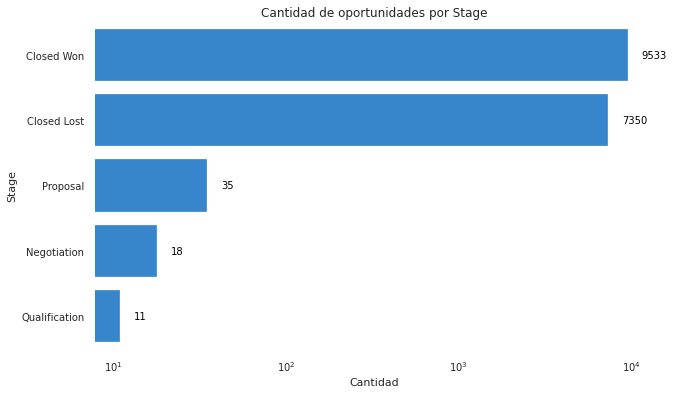
\includegraphics[width=0.7\textwidth]{images/bp_cantidad_opp_por_stage_log.png}
\cprotect\caption{\label{fig:bp_cant_opp_por_stage}Cantidad de oportunidades por \textit{Stage}}
\end{figure}

\subsection{\textit{Stages} en el tiempo}
Además contamos con información temporal de cuándo sucede la oportunidad, pudiendo así ver en el gráfico de la figura \ref{fig:bp_cantidad_de_oportunidades_por_cuatrimestre} cómo fue evolucionando la cantidad a lo largo de los años segmentado por cuatrimestres. Algo para considerar es que la información que se cuanta desde el primer cuatrimestre del 2019 hacia adelante es muy inferior a las años que le preceden. Esto se puede deber que se tiene un subconjunto del \textit{dataset} original, o bien no se cuentan oportunidades posteriores al susodicho cuatrimestre. Es más probable que la primera opción sea más certera, pues los dos años posteriores se cuenta con muy poca información.

\begin{figure}[H]
\centering
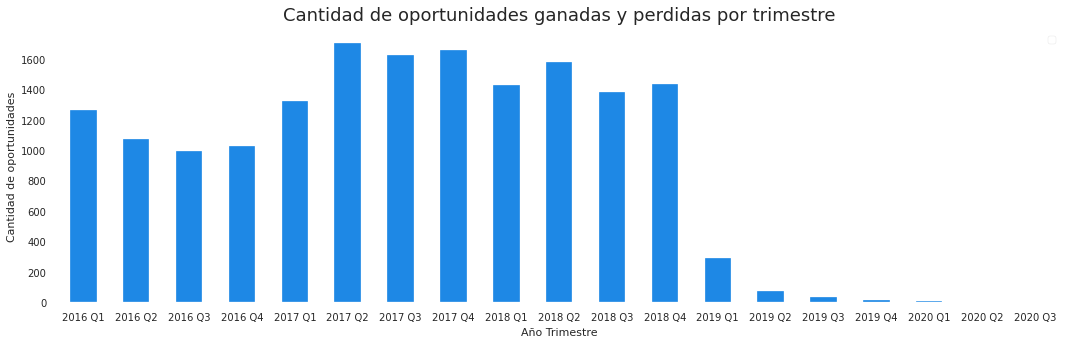
\includegraphics[width=0.8\textwidth]{images/bp_cantidad_de_oportunidades_por_cuatrimestre.png}
\cprotect\caption{\label{fig:bp_cantidad_de_oportunidades_por_cuatrimestre}Cantidad de oportunidades por año-cuatrimestre. }
\end{figure}

Una vez visto las cantidades netas, en el gráfico \ref{fig:bp_oportunidades_ganadas_y_perdidas_por_cuatrimestre} se pueden ver las oportunidades que nos interesa estudiar, que son aquellas que fueron cerradas, exitosamente o no. Era de esperar que el patrón de faltantes de datos del cuatrimestre primero de 2019 hacia delante se mantuviera. Por lo que se ve en el gráfico, solamente en los primeros dos cuatrimestre (que se tienen datos) se obtuvo un \textit{win-ratio} ($\rho_w = \frac{|O_w|}{|O_T|}$) menor al 0.5, en los cuatrimestres posteriores, se fue superando ese número, exceptuando, nuevamente, al cuatrimestre primero de 2019, que para este caso en particular no se saca conclusiones, ya que, por lo mencionado anteriormente, no se está seguro de la completitud de los datos.

\begin{figure}[H]
\centering
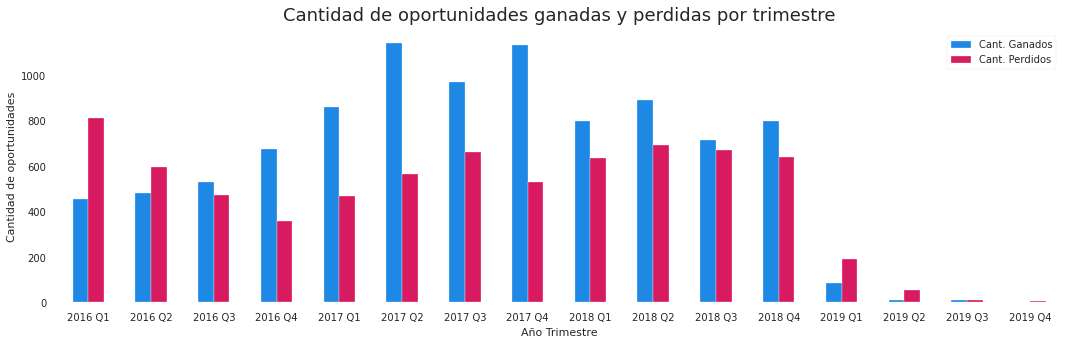
\includegraphics[width=0.8\textwidth]{images/bp_oportunidades_ganadas_y_perdidas_por_cuatrimestre.png}
\cprotect\caption{\label{fig:bp_oportunidades_ganadas_y_perdidas_por_cuatrimestre} Cantidad de oportunidades ganadas y perdidas por año-cuatrimestre. }
\end{figure}

\subsection{\textit{Stages} por región}
Para hilar más fino sobre los datos, en la figura \ref{fig:bp_oportunidades_ganadas_y_perdidas_por_region} analiza la variable de cantidad de oportunidades ganadas y perdidas, segmentado por región. \textit{Japón} cuenta con mayor \textit{win-ratio}, es decir, las oportunidades en esa región suelen ser más exitosas comparadas con otras regiones. En contraparte, en la región \texit{Americas}, se tiene el efecto inverso, aunque en menor medida. Finalmente, la región \textit{Medio Oriente}, también cuenta con un bajo \textit{win-rate}, puede llegar a ser apresurado sacar conclusiones en base a este dato, ya que como se ve en relación a los demás, esta región cuenta con menos oportunidades que las demás.

\begin{figure}[H]
\centering
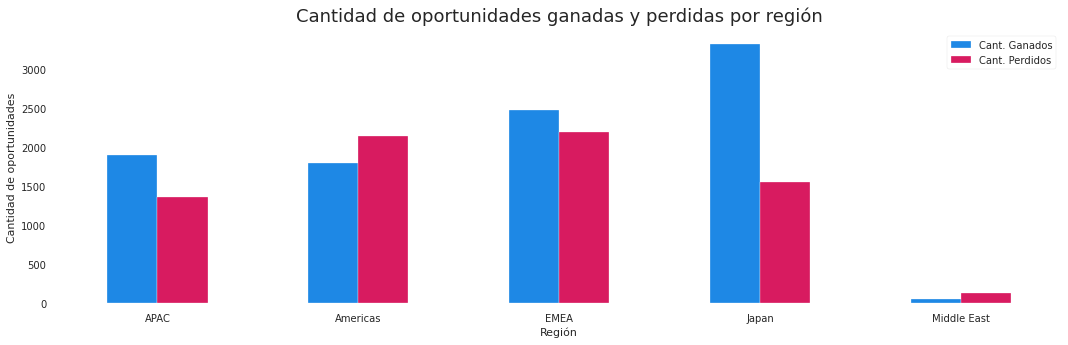
\includegraphics[width=0.9\textwidth]{images/bp_oportunidades_ganadas_y_perdidas_por_region.png}
\cprotect\caption{\label{fig:bp_oportunidades_ganadas_y_perdidas_por_region} Cantidad de oportunidades ganadas y perdidas por región. }
\end{figure}

\section{Tiempos de entrega}
En base a la información provista \verb|Planned_Delivery_Start_Date| y \verb|Planned_Delivery_End_Date|, se calcula el tiempo (en días) que duraría la entrega. Al explorar esta nueva variable, se pudo notar una anormalidad, una de las oportunidades estaba programada con fecha \verb|2208-12-31| que carece de sentido en este contexto.

Haciendo el primer análisis de la duración de las entregas, se calcula el promedio de la duración de envíos (para los casos \verb|Closed Won|), como se muestra en la figura \ref{fig:promedio_tiempo_entrega_region}, \textit{Japón} tiene el promedio más bajo, es decir realiza entregas más rápido que las demás regiones. Explorando los datos, se observó que muchas de las entregas de \textit{Japón} están programadas para ser entregadas en el mismo día, es decir que \verb|Planned_Delivery_Start_Date| es igual a \verb|Planned_Delivery_End_Date|, esto puede ser efectivamente así, o puede ser un error de carga. Al no poder confirmarlo, se asumirá que esta información es correcta.

\begin{figure}[H]
\centering
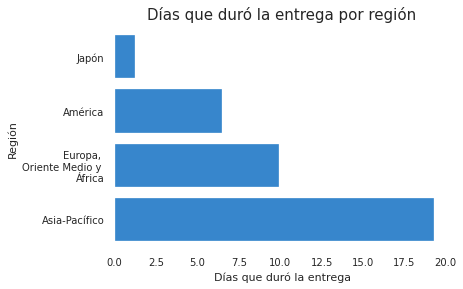
\includegraphics[width=0.5\textwidth]{images/bp_tiempo_promedio_tiempo_entrega_por_region.png}
\cprotect\caption{\label{fig:promedio_tiempo_entrega_region}Tiempo promedio de entrega por región}
\end{figure}

A su vez, cada oportunidad, tiene asignado un término de entrega, este es una categoría y puede representar algún tipo de logística asociada (por ejemplo, un envío internacional o relacionado con las dimensiones del equipo en cuestión). En la figura \ref{fig:bp_cantidad_opp_por_termino_de_entrega} se muestran el número de oportunidades por término de envío.
\begin{figure}[H]
\centering
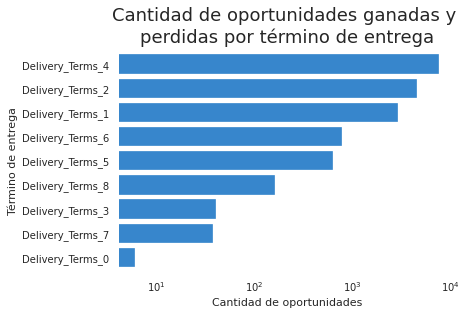
\includegraphics[width=0.6\textwidth]{images/bp_cantidad_opp_por_termino_de_entrega.png}
\cprotect\caption{\label{fig:bp_cantidad_opp_por_termino_de_entrega} Cantidad de oportunidades por término de entrega. }
\end{figure}

Como se ve en la figura \ref{fig:bp_oportunidades_ganadas_y_perdidas_por_termino_de_entrega}, si bien no aporta información significativa, si se puede ver que \verb|Delivery_Terms_1| es el único con un \textit{win-rate} menor al 0.5, aunque no por mucho. Para evitar obtener resultados que puedan llevar a conclusiones erróneas, se hace el análisis sobre aquellas que tengan por lo menos una cierta cantidad límite de oportunidades, apelando a la ecuación de \textit{de Moivre} \cite{la_ecuacion_mas_peligrosa}.
\begin{figure}[H]
\centering
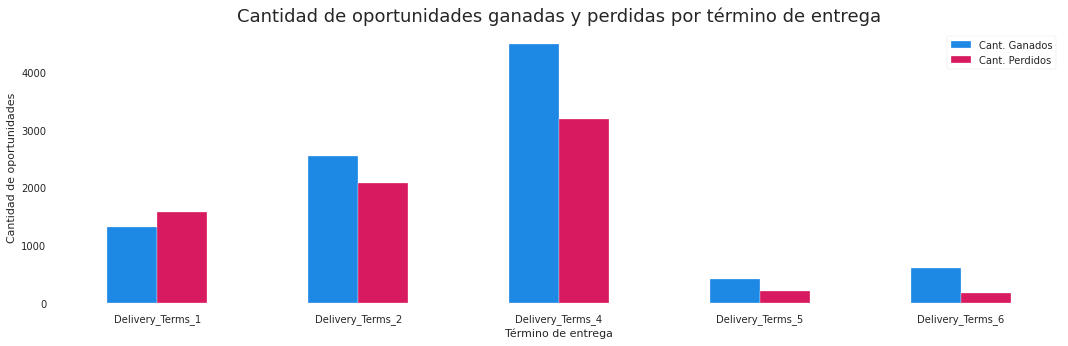
\includegraphics[width=0.9\textwidth]{images/bp_oportunidades_ganadas_y_perdidas_por_termino_de_entrega.png}
\cprotect\caption{\label{fig:bp_oportunidades_ganadas_y_perdidas_por_termino_de_entrega} Cantidad de oportunidades ganadas y perdidas por término de entrega. }
\end{figure}


\subsection{Tiempos de entrega a través del tiempo}
Una vez obtenido este resultado, se estudia, cómo fue evolucionando este promedio en el tiempo (sería razonable que en un comienzo, por falta de logística, las entregas se demoraran más o bien, a medida que avanza el tiempo, la demanda aumente, retrasando así las entregas). Al ver el gráfico en la figura \ref{fig:line_promedio_tiempo_entrega_region}, se observa que tanto en \textit{Medio Oriente} como en \textit{América}, el promedio fue aumentando, apoyando la hipótesis del aumento en la demanda, en cambio en \textit{Asia-Pacífico} disminuyó en el último tiempo. Por su parte, tanto \textit{Europa, Oriente Medio y África} y \textit{Japón} se mantuvo aparentemente constante a lo largo del tiempo. En particular, no se logra apreciar la evolución de estos últimos por el desbalance que generan las demás regiones, con lo cual, se realiza el análisis por separado en el gráfico de la figura \ref{fig:promedio_tiempo_entrega_region_japon_EMEA}

\begin{figure}[H]
\centering
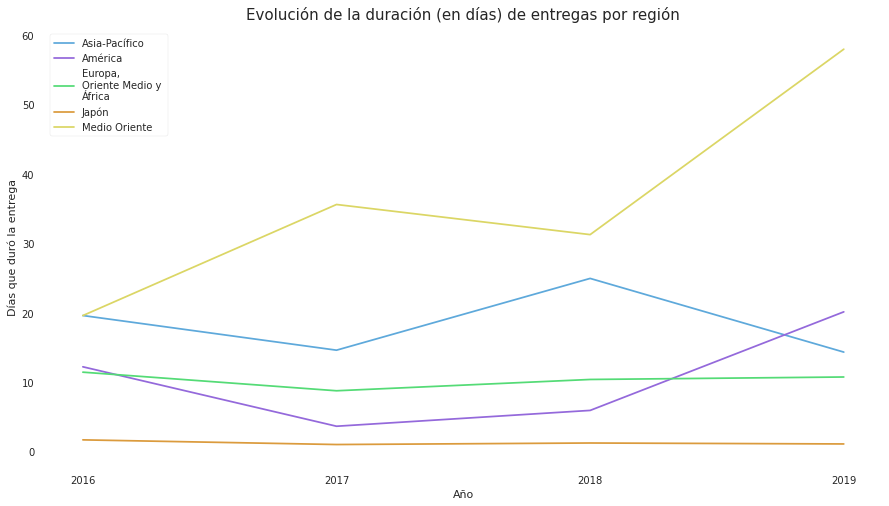
\includegraphics[width=0.7\textwidth]{images/lp_ev_duracion_tiempo_entrega_por_region.png}
\cprotect\caption{\label{fig:line_promedio_tiempo_entrega_region}Tiempo promedio de entrega por región a través de los años.}
\end{figure}

\begin{figure}[H]
\centering
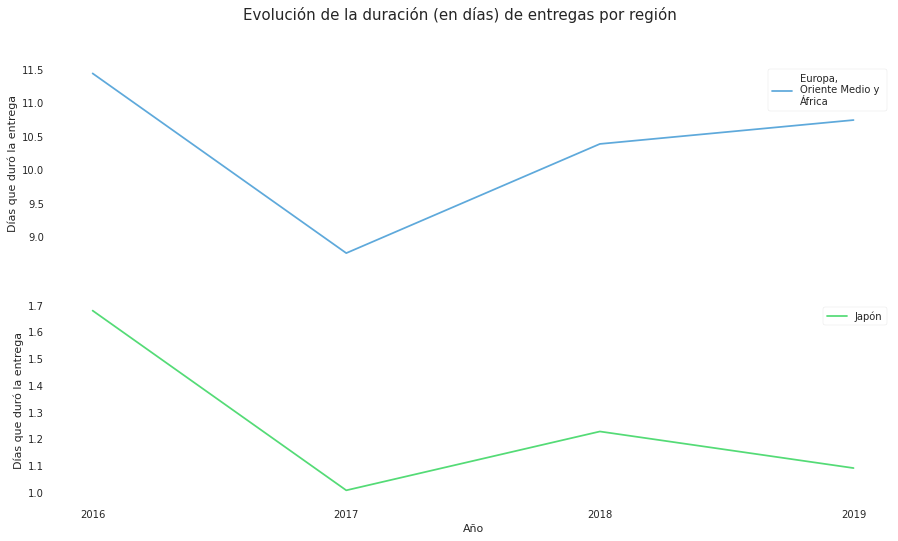
\includegraphics[width=0.7\textwidth]{images/lp_ev_duracion_tiempo_entrega_por_region_japon_emea.png}
\cprotect\caption{\label{fig:promedio_tiempo_entrega_region_japon_EMEA}Tiempo promedio de entrega en \textit{Japón} y \textit{EMEA} a través de los años.}
\end{figure}

\subsection{Causas del tiempo de entrega}
Una de las razonas de la demora en la entrega puede deberse, por ejemplo, al tamaño de los equipos, para estimar esto se emplea la referencia del dato \verb|TRF| (Toneladas de refrigeración), donde a mayor \verb|TRF| se trata de un equipo de mayor tamaño. A su vez, esto puede estar relacionado con la probabilidad de éxito de la oportunidad, ya que en primer lugar, es difícil vender un equipo grande (con alto \verb|TRF|), es probable que el cliente cancele una oportunidad si considera que el tiempo de entrega no le es útil para su caso de uso, y finalmente una combinación de ambas. En la figura \ref{fig:scatter_dur_envio_trf}, si bien, se puede ver que la mayoría de las oportunidades excediendo cierto valor de \verb|TRF| y un valor de duración del envío, son oportunidades que fueron perdidas, esto no necesariamente es algo concluyente, ya que la mayoría del total de oportunidades se concentra en el rango opuesto.

\begin{figure}[H]
\centering
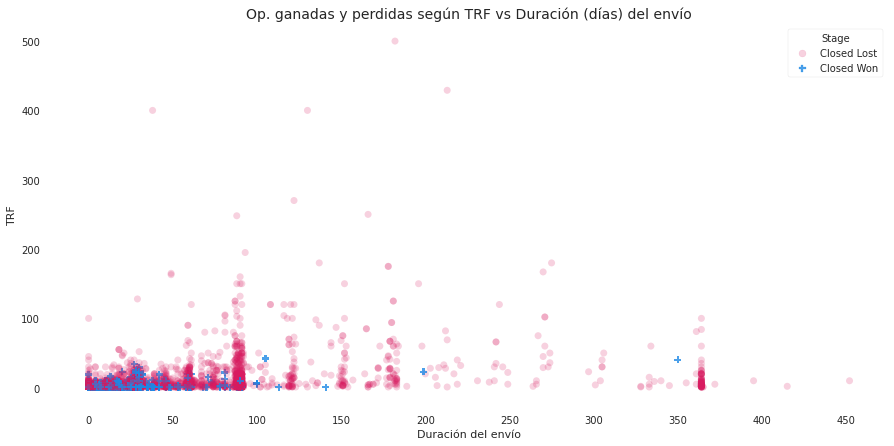
\includegraphics[width=0.7\textwidth]{images/scatter_dur_envio_trf.png}
\cprotect\caption{\label{fig:scatter_dur_envio_trf} Tiempo de entrega contra el TRF del equipo. }
\end{figure}

Partiendo de este gráfico, se realizan los gráficos de la figura \ref{fig:scatter_dur_envio_trf_region}, realizando el mismo análisis pero sobre cada región, agregando un estudio local sobre un rango más acotado para ver los datos que no entran en el análisis anterior.
\begin{figure}[H]
\centering
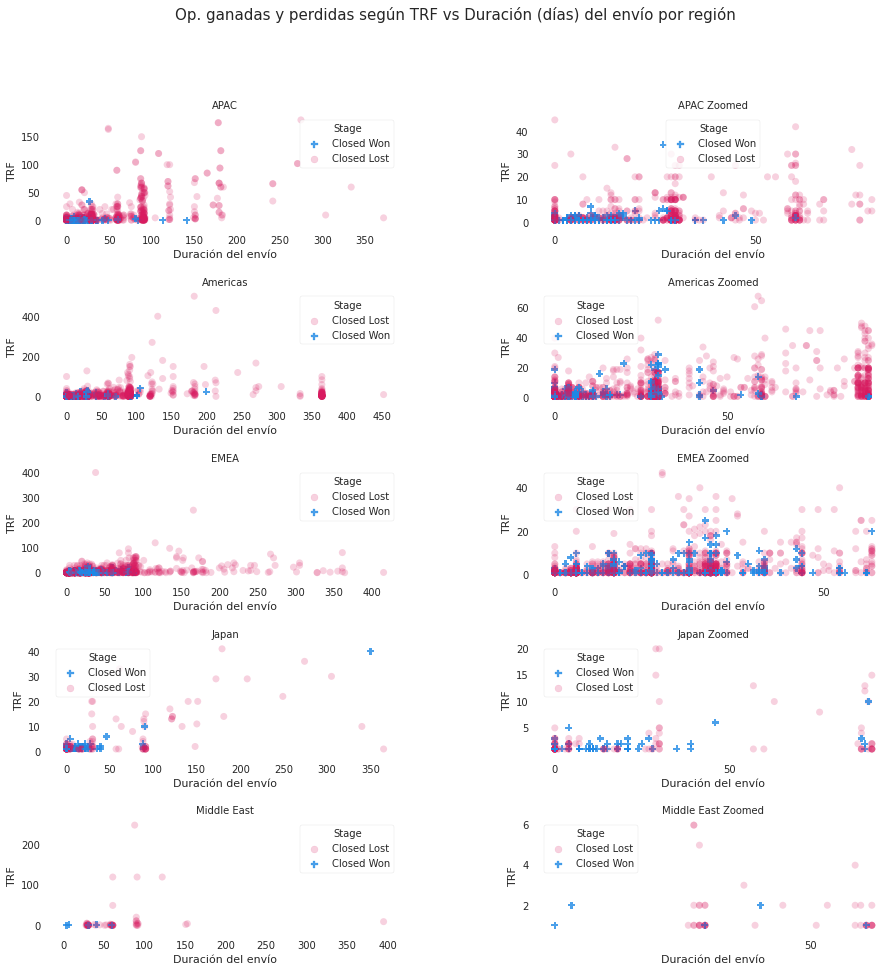
\includegraphics[width=0.7\textwidth]{images/scatter_dur_envio_trf_region.png}
\cprotect\caption{\label{fig:scatter_dur_envio_trf_region} Tiempo de entrega contra el TRF del equipo por región. }
\end{figure}

En base al grafico de la figura \ref{fig:scatter_dur_envio_trf_region} no se saca ninguna conclusión de la región \textit{Medio Oriente}, pues hay pocos datos. En cuanto a \textit{APAC} y \textit{Americas} son las regiones donde se realizan los pedidos de equipos con mayor \verb|TRF|, que se ve que en general, se cumple con la hipótesis de a mayor \verb|TRF| (mayor el equipo) es más probable que la oportunidad no sea ganada. En cuanto a el tiempo de entrega, se puede notar un quiebre, alrededor de de los 100 días, donde a partir de ahí son oportunidades perdidas.

Algo para notar, que se ve mejor en las regiones \textit{EMEA} y \textit{Americas} (en el gráfico aumentado), es que aproximadamente hasta los 35-40 días de entregas, se ven oportunidades exitosas, aún teniendo un \verb|TRF| alto, desde ahí, esa tendencia tiende a invertirse.

En la figura \ref{fig:vi_distribucion_duracion_dias}, se reafirma que desde este parámetro, duración del envío, nos puede ayudar a descartar aquellos que superen cierto límite. Es notable ver, por ejemplo, en \textit{APAC} que a partir de los 50 días, son mayoritariamente ventas perdidas. En contraposición, no es clara ninguna conclusión sobre oportunidades que estén abajo de ese límite.

\begin{figure}[H]
\centering
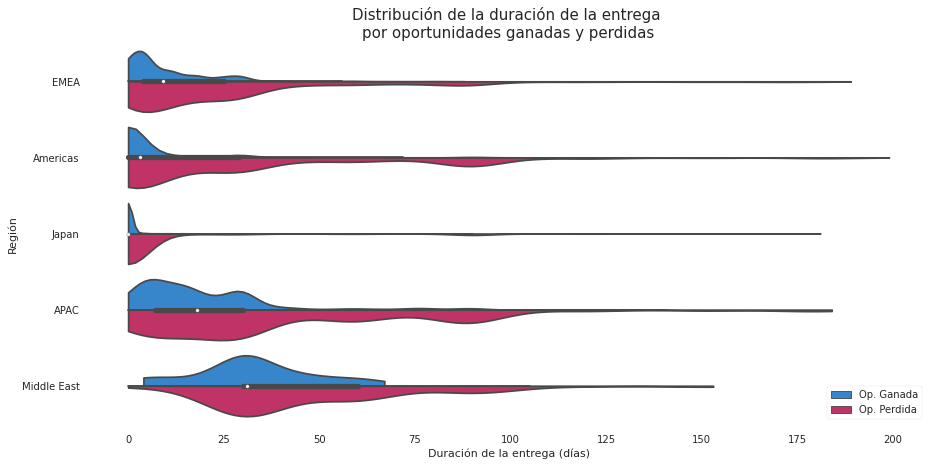
\includegraphics[width=0.9\textwidth]{images/vi_distribucion_duracion_dias.png}
\cprotect\caption{\label{fig:vi_distribucion_duracion_dias} Distribución tiempo de entrega por región. }
\end{figure}

\section{Tipo de familia de productos}
Una de las características de los productos, es que cuenta con un `tipo de familia'. Se desea hacer el análisis para ver si alguna de las familias cuanta con un mayor \textit{win-ratio}  respecto a las demás. En la figura \ref{fig:bp_familia_de_productos_ordenadas_winratio} se muestran todas las familias (que superen un número de oportunidades) ordenadas según su \textit{win-ratio}, está claro que las familias que se encuentran más arriba son aquellas con mayor $\rho_w$.

\begin{figure}[H]
\centering
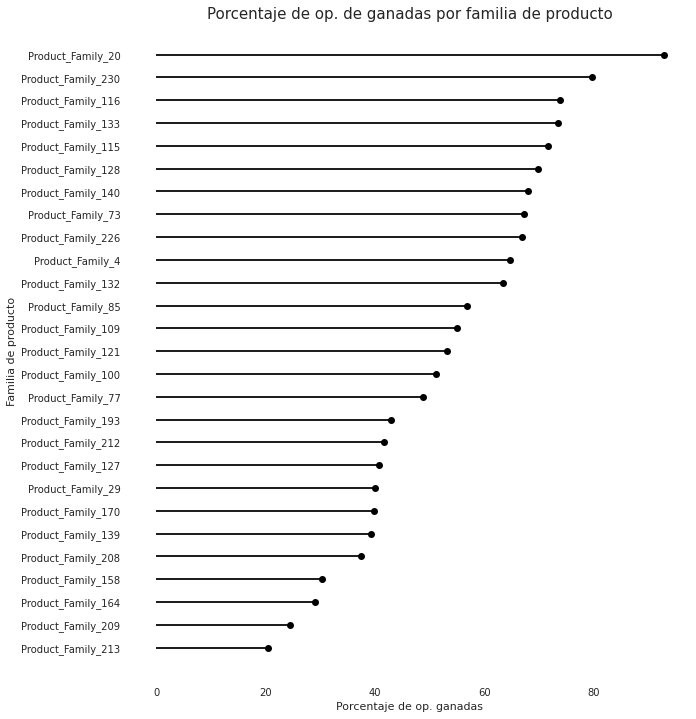
\includegraphics[width=0.9\textwidth]{images/bp_familia_de_productos_ordenadas_winratio.png}
\cprotect\caption{\label{fig:bp_familia_de_productos_ordenadas_winratio} Familias de producto ordenadas por \textit{win-ratio}. }
\end{figure}

Una vez obtenido este resultado general, en la figura \ref{fig:bp_top_familia_de_productos_con_mas_winratio} se hace foco sobre las primeras, viendo así que, no necesariamente, las que más oportunidades tienen, les va mejor. Si por el contrario, vemos en la figura \ref{fig:bp_top_familia_de_productos_con_menos_winratio} las familias con peor ratio. Desde acá se puede postular que dependiendo el tipo de familia de producto (y lo que ello signifique dentro de la denominación del producto) la probabilidad de éxito puede verse modificada por esta variable.

\begin{figure}[H]
\centering
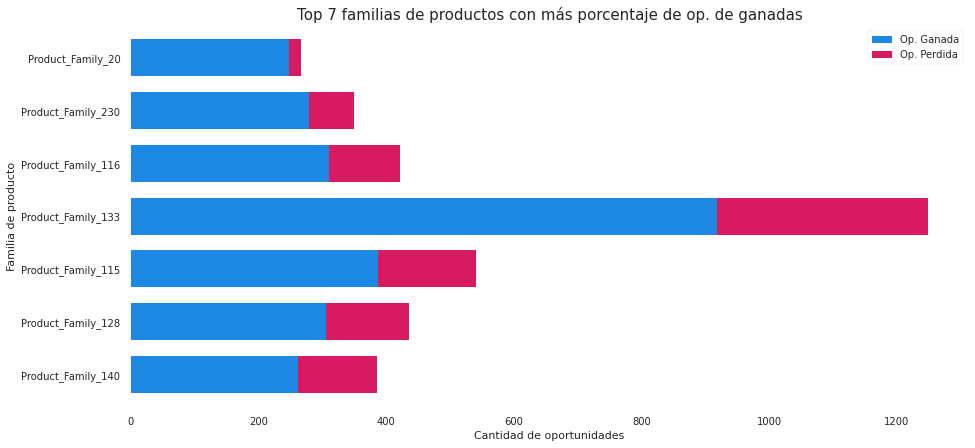
\includegraphics[width=0.9\textwidth]{images/bp_top_familia_de_productos_con_mas_winratio.png}
\cprotect\caption{\label{fig:bp_top_familia_de_productos_con_mas_winratio} Top 7 familias de producto con mayor \textit{win-ratio}. }
\end{figure}

\begin{figure}[H]
\centering
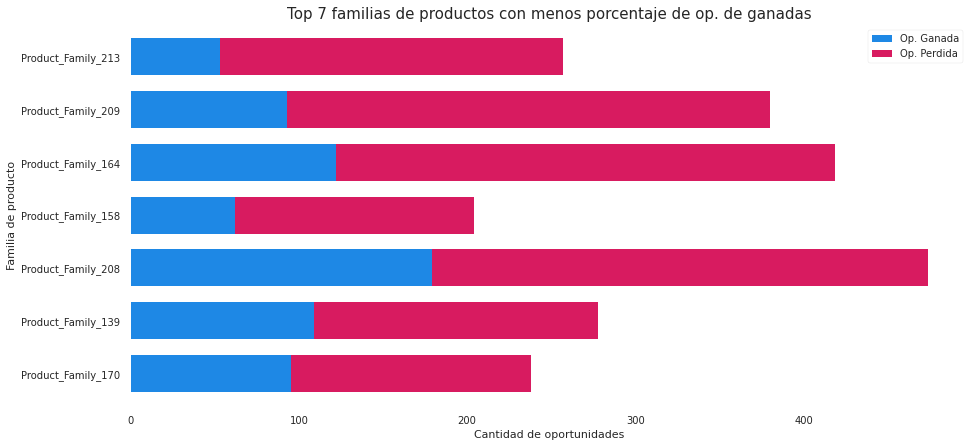
\includegraphics[width=0.9\textwidth]{images/bp_top_familia_de_productos_con_menos_winratio.png}
\cprotect\caption{\label{fig:bp_top_familia_de_productos_con_menos_winratio} Top 7 familias de producto con menor \textit{win-ratio}. }
\end{figure}

\section{Personas}
Cada oportunidad tiene asociada un \textit{dueño de oportunidad} y  \textit{dueño de cuenta}, estos conjuntos no son necesariamente excluyente. Haciendo un análisis sobre estas dos variables, en la figura \ref{fig:ps_personas_GLOBAL} vemos que hay un empleado predominantes, \verb|Person_name_50|, con un \textit{win-ratio} ($\rho_w$) superior al 0.5, seguido, se encuentran \verb|Person_name_13|, \verb|Person_name_8| y \verb|Person_name_18|. Estas primeras cuatro personas, parecería que trabajan mayoritariamente solas en cada oportunidad, hay poca interacción con las demás, un excepción a esto es la persona \verb|Person_name_43|, que cierto porcentaje de oportunidades ganadas fueron interactuando con la \verb|Person_name_19|. Es notable destacar que la persona \verb|Person_name_3| (dentro de las personas con mayor venta), tiene peor \textit{win-ratio}.

\begin{figure}[H]
\centering
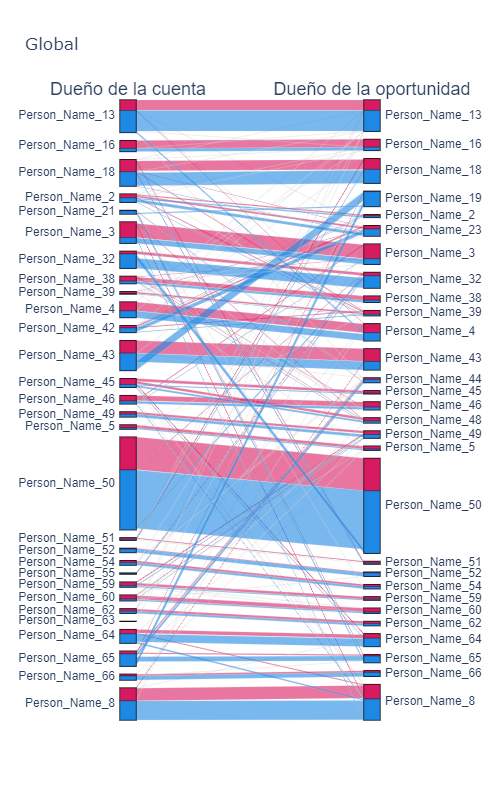
\includegraphics[width=0.7\textwidth]{images/ps_personas_GLOBAL.png}
\cprotect\caption{\label{fig:ps_personas_GLOBAL} Relaciones entre personas diferenciando oportunidades ganadas y perdidas (global).}
\end{figure}

\subsection{Relaciones de personas por región}
Un problema notable del gráfico de la figura \ref{fig:ps_personas_GLOBAL}, es que aquellas personas con menos oportunidades que las principales, se ven opacadas. Por eso se hace un análisis segmentado por región.

En la figura \ref{fig:bp_cantidad_de_dueños_de_oportunidad_por_region} se muestra la cantidad de \textit{dueños de oportunidad} que hay por cada región.

\begin{figure}[H]
\centering
\includegraphics[width=0.5\textwidth]{images/bp_cantidad_de_dueños_de_oportunidad_por_region.png}
\cprotect\caption{\label{fig:bp_cantidad_de_dueños_de_oportunidad_por_region} Cantidad de \textit{dueños de oportunidad} por región}
\end{figure}
Aparentemente los datos en \textit{Medio Oriente} son significativamente inferiores a las demás, con lo cual este análisis no lo va a tener en cuenta.

Una vez tenido un vistazo global, en la figura \ref{fig:box_distribucion_cant_ventas_duenos_opp_por_region}, se analiza cómo se distribuyen estos \textit{dueños de oportunidad} dentro de cada una de las regiones según su cantidad de ventas. Aunque se observa una gran varianza en \textit{Americas}, concentra el mayor promedio por persona.

\begin{figure}[H]
\centering
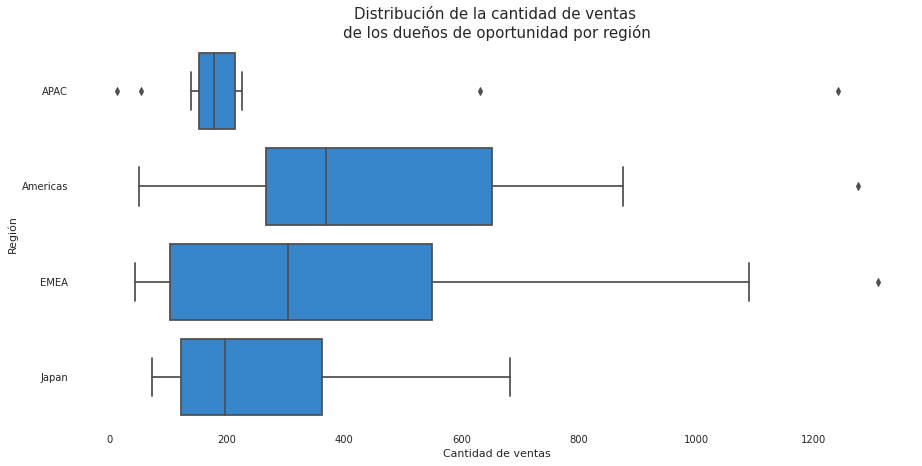
\includegraphics[width=0.8\textwidth]{images/box_distribucion_cant_ventas_duenos_opp_por_region.png}
\cprotect\caption{\label{fig:box_distribucion_cant_ventas_duenos_opp_por_region} Distribución de las personas según su \textit{win-ratio} por región. }
\end{figure}

En base al gráfico de la figura \ref{fig:box_distribucion_cant_ventas_duenos_opp_por_region}, ahora se quiere conocer cómo se distribuyen estas personas, en particular, cómo se distribuyen según su \textit{win-ratio}, obteniendo así el gráfico de la figura \ref{fig:vi_distribucion_duenos_opp_por_win_ratio}. Se observa que las regiones con mayor \textit{win-ratio} se concentran en \textit{Japón} y \textit{APAC}, mientras que en \textit{EMEA}  y \text{Americas} se encuentran un poco por debajo de las mencionadas. Nuevamente, por la falta de datos en \textit{Middle East}, es difícil tomar conclusiones en dicha región. Algo para notar, en la región de \textit{Japón}, no se cuenta con información significante de dueños de oportunidad con \textit{win-ratio} bajo.

\begin{figure}[H]
\centering
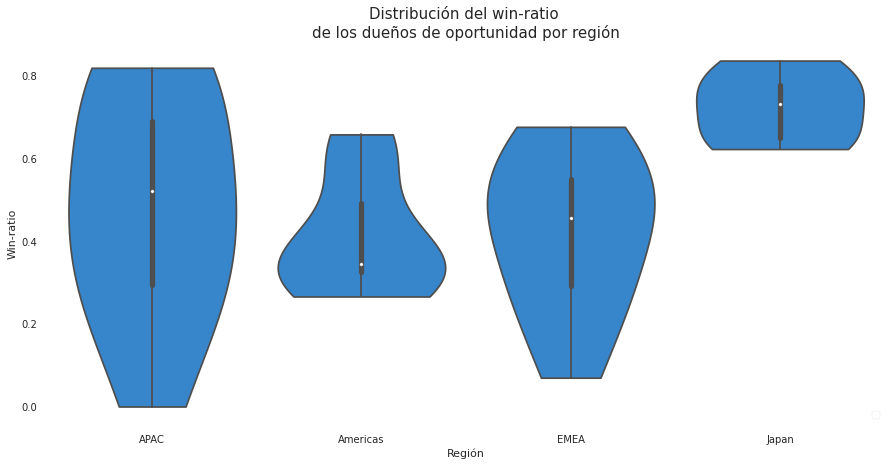
\includegraphics[width=0.7\textwidth]{images/vi_distribucion_duenos_opp_por_win_ratio_2.png}
\cprotect\caption{\label{fig:vi_distribucion_duenos_opp_por_win_ratio} Distribución de las personas según su \textit{win-ratio} por región. }
\end{figure}

\begin{figure}[H]
\centering
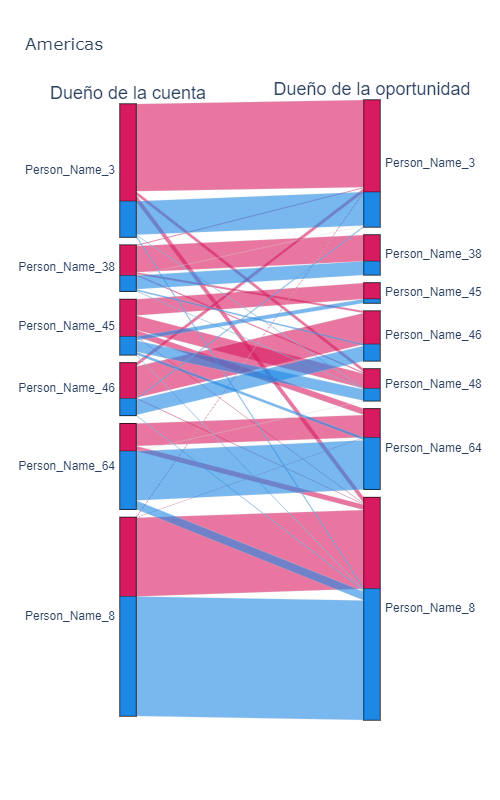
\includegraphics[width=0.5\textwidth]{images/ps_personas_america.png}
\cprotect\caption{\label{fig:ps_personas_america} Relaciones entre personas diferenciando oportunidades ganadas y perdidas (Americas).}
\end{figure}


En el gráfico de \textit{Americas} de la figura \ref{fig:ps_personas_america}, se ve que las personas con mayores ventas son \verb|Person_name_8| (uno de los principales globales), \verb|Person_name_64| y \verb|Person_name_3|, este último con un bajo \textit{win-ratio}. Las demás personas en esta región no superan el \textit{win-ratio} de 0.5.

\begin{figure}[H]
\centering
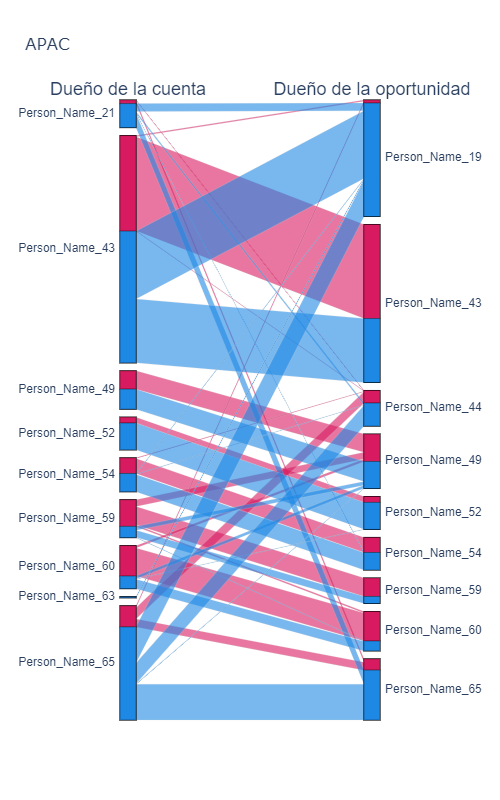
\includegraphics[width=0.7\textwidth]{images/ps_personas_APAC.png}
\cprotect\caption{\label{fig:ps_personas_APAC} Relaciones entre personas diferenciando oportunidades ganadas y perdidas (APAC).}
\end{figure}

Para la región \textit{APAC} (figura \ref{fig:ps_personas_APAC}), se ve un \textit{win-ratio} mayor en promedio y además se puede ver como las distintas personas tienden a cooperar más entre ellos. Esto último no es el causante del primero, ya que se puede ver que por ejemplo la persona \verb|Person_name_59| tiene un alto grado de cooperación pero aún así un bajo \textit{win-ratio}.


\begin{figure}[H]
\centering
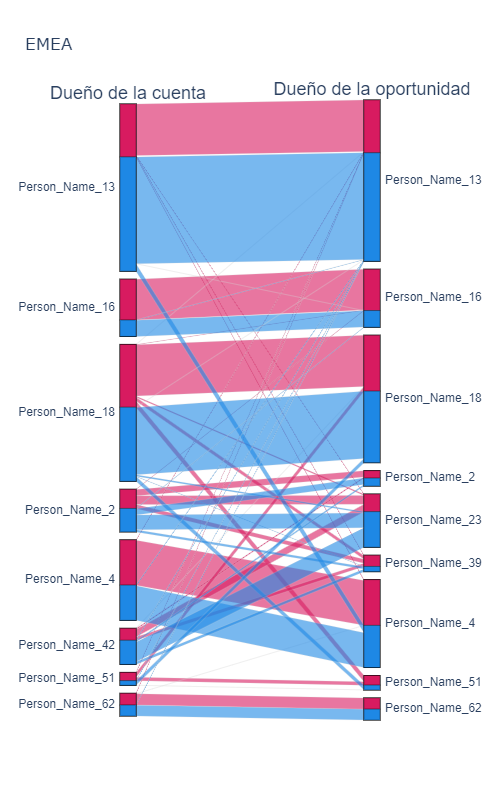
\includegraphics[width=0.7\textwidth]{images/ps_personas_EMEA.png}
\cprotect\caption{\label{fig:ps_personas_EMEA} Relaciones entre personas diferenciando oportunidades ganadas y perdidas (EMEA).}
\end{figure}

En la región de \textit{EMEA} (ver figura \ref{fig:ps_personas_EMEA}), se encuentra dos de las personas con mayor cantidad de ventas mundial, \verb|Person_name_13| y \verb|Person_name_18|. En esta región en particular, se nota que hay personas con pocas ventas asociadas, pero que intervinieron con muchas personas, y esto sucede tanto del lado \textit{dueño de cuenta} como \textit{dueño de oportunidad}.

\begin{figure}[H]
\centering
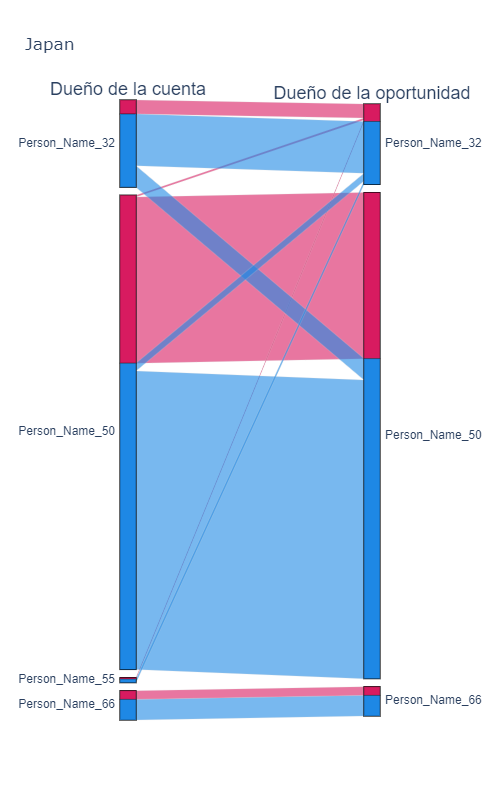
\includegraphics[width=0.7\textwidth]{images/ps_personas_japan.png}
\cprotect\caption{\label{fig:ps_personas_japan} Relaciones entre personas diferenciando oportunidades ganadas y perdidas (Japón).}
\end{figure}

En la región de \textit{Japón} (figura \ref{fig:ps_personas_japan}), se cuentan con menor cantidad de personas con ventas significativas, con lo cual es un tanto peligroso sacar conclusiones, pero algo a destacar es que tiene presente a la persona con mayores ventas asociadas mundiales, \verb|Person_name_50|, que además cuenta con un alto \textit{win-ratio}. Esto último es algo que se mantiene dentro de las personas que están siendo analizadas en esta región.

Finalmente, pera la región \textit{Medio Oriente}, no se cuenta con información suficiente para realizar algún análisis de este tipo.


\section{Conclusiones}
% TODO: Conclusiones





\subsection{Oportunidades de mejoras}
A lo largo del trabajo práctico fueron surgiendo inconvenientes, ya sea falta de tiempo o de conocimiento, generaron posibles oportunidades de mejoras.
\subsubsection{Entendimiento mayor del modelo del negocio}
Al contar con información un tanto críptica, la cual era difícil de asociar algo tangible, fue difícil interpretar los datos, desaprovechando así posibles variables importantes para la predicción de oportunidad de éxito. La mejora de la calidad del análisis se podría lograr tratando de obtener más reglas de negocios que están asociadas con los datos provistos.

\subsubsection{Reducción de consumo de memoria}
Cuando se empezó a analizar los datos desde una primera vista, se pudo fue viendo qué variables eran categóricas y cuales no. Las variables categóricas nos permiten ahorrar espacio en memoria que ocupa el \textit{dataframe} al reducir la información duplicada. Los atributos que fueron pensados como categóricos fueron:

\begin{itemize}
    \item \verb|ASP_(converted)_Currency|
    \item \verb|Stage|
    \item \verb|Region|
    \item \verb|Territory|
    \item \verb|Pricing, Delivery_Terms_Quote_Appr|
    \item \verb|Pricing, Delivery_Terms_Approved|
    \item \verb|Bureaucratic_Code_0_Approval|
    \item \verb|Bureaucratic_Code_0_Approved|
    \item \verb|Bureaucratic_Code|
    \item \verb|Source|
    \item \verb|Billing_Country|
    \item \verb|Account_Owner|
    \item \verb|Opportunity_Owner|
    \item \verb|Account_Type|
    \item \verb|Opportunity_Type|
    \item \verb|Quote_Type|
    \item \verb|Delivery_Terms|
    \item \verb|Brand|
    \item \verb|Product_Type|
    \item \verb|Size|
    \item \verb|Product_Category_B|
    \item \verb|Currency|
    \item \verb|Last_Modified_By|
    \item \verb|Product_Family|
    \item \verb|Product_Name|
    \item \verb|Month|
    \item \verb|Delivery_Quarter|
    \item \verb|Total_Amount_Currency|
    \item \verb|Total_Taxable_Amount_Currency|
\end{itemize}

Que originalmente ocupaba algo asó como 5.9 MB.
\begin{verbatim}
    dtypes: float64(3), int64(8), object(35)
    memory usage: 5.9+ MB
\end{verbatim}

Y pasó a ocupar menos de la mitad:
\begin{verbatim}
    dtypes: category(29), datetime64[ns](3), float64(3), int64(4), object(8)
    memory usage: 2.9+ MB
\end{verbatim}

Esto se logró pasando estos atributos de \verb|object| a \verb|pd.Categorical|. El inconveniente con esta modificación fue que generó dificultades para poder graficar, con lo cual se descartó este cambio para simplificar la codificación.

\subsubsection{Mejoras de código}
Para realizar cada uno de los gráficos, se fueron tomando bloques independientes en una \textit{notebook} de \textit{Google Colab} \footnote{Google Colab \href{https://colab.research.google.com/}{https://colab.research.google.com/}}, lo que hizo que haya mucho código desordenado y repetido.

\newpage
\appendix
\section{Ejecución del \text{script} que genera los gráficos}
Para poder correr el \texit{script} que genera el análisis y los gráficos, primero hay que instalar las librerías necesarias, se puede hacer mediante la herramienta \verb|pip| \footnote{Herramienta \verb|pip|: \href{https://pypi.org/project/pip/}{https://pypi.org/project/pip/}} con el siguiente comando:

\begin{verbatim}
    pip install -r requirements.txt
\end{verbatim}
Para realizar realizar una instalación más ordenada y sin tener conflicto de versiones es recomendable usar un entorno virtual \footnote{Entorno virtual de python (venv): \href{https://docs.python.org/3/library/venv.html}{https://docs.python.org/3/library/venv.html}}
Una vez finalizada la instalación, para ejecutar el programa:
\begin{verbatim}
    python tp_datos_2c2020.py
\end{verbatim}

Si se quiere evitar la parte de instalación se puede ejecutar desde la herramienta \textit{Google Colab} \footnote{Google Colab \href{https://colab.research.google.com/}{https://colab.research.google.com/}}.

\section{Elección de colores}
Gran parte del informe, se encuentra con la misma gama cromática, estos colores son (en formato hex) `\verb|#1E88E5|' \tikz{\draw[fill={rgb,255:red,30; green,136; blue,229},line width=0.2pt]  circle(1ex);}, generalmente asignado a oportunidades ganadas o resultados neutros, y `\verb|#D81B60|' \tikz{\draw[fill={rgb,255:red,216; green,27; blue,96},line width=0.2pt]  circle(1ex);} generalmente usado para denotar oportunidades perdidas. Se hace esta elección, frente a las combinaciones de verde-rojo (que suele representar lo mismo), para poder facilitar el análisis para personas con problemas de daltonismo \cite{color_blind_visu}. Como se puede ver en la figura \ref{fig:bp_colores} se presentan dos gráficos con dos paletas de colores distintas, la primera es rojo-verde, la segunda es la propuesta que se usó en el trabajo. En su contraparte, en la figura \ref{fig:bp_colores_converted} se encuentra la misma imagen, pasada por un filtro de simulación de problemas de vista \cite{simulador_problemas_visuales}.

\begin{figure}[H]
\centering
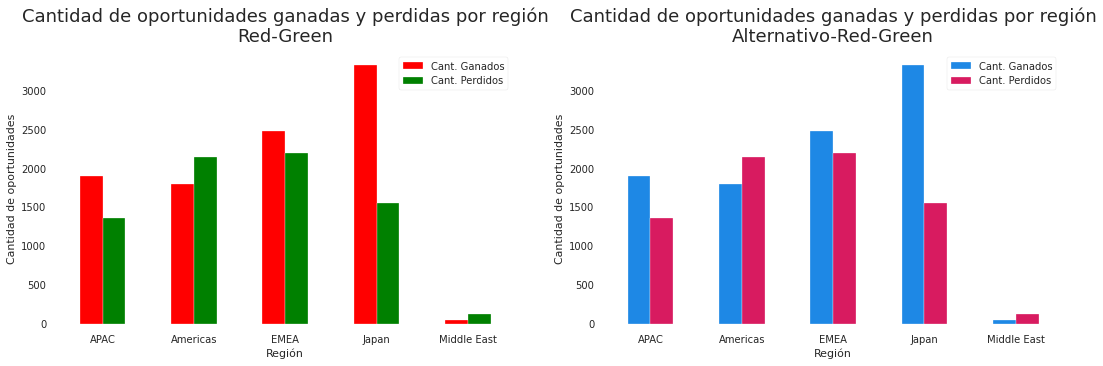
\includegraphics[width=0.8\textwidth]{images/bp_colores.png}
\cprotect\caption{\label{fig:bp_colores} Barplot original.}
\end{figure}

\begin{figure}[H]
\centering
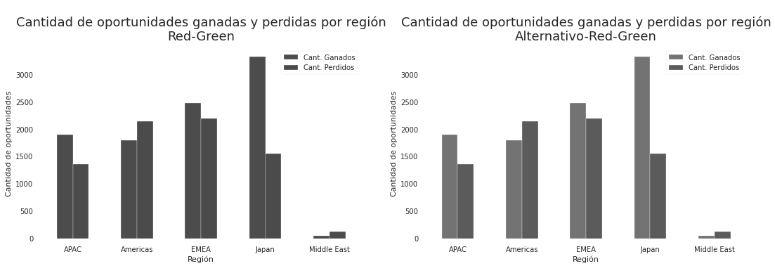
\includegraphics[width=0.8\textwidth]{images/bp_colores_converted.png}
\cprotect\caption{\label{fig:bp_colores_converted} Barplot como lo vería una persona con vista monocromática. }
\end{figure}

\newpage

\begin{thebibliography}{9}

\bibitem{la_ecuacion_mas_peligrosa}
\cprotect\textit{La ecuación más peligrosa [En]}. 
\href {https://www.americanscientist.org/article/the-most-dangerous-equation}{
https://www.americanscientist.org/article/the-most-dangerous-equation
}

\bibitem{color_blind_visu}
\cprotect\textit{Alternativas de colores para rojo-verde [En]}. 
\href {https://www.visualisingdata.com/2019/08/five-ways-to-design-for-red-green-colour-blindness/}{
https://www.visualisingdata.com/2019/08/five-ways-to-design-for-red-green-colour-blindness/
}

\bibitem{simulador_problemas_visuales}
\cprotect\textit{Simulador de distintos tipos de daltonismo}. 
\href {https://www.color-blindness.com/coblis-color-blindness-simulator/}{
https://www.color-blindness.com/coblis-color-blindness-simulator/
}
\end{thebibliography}


\end{document}